% Niveau :      PCSI
% Discipline :  Mécaflu
%Mots clés :    

\begin{exercise}{Atmosphère polytropique}{2}{Sup, Spé}
{Statique des fluides, Thermodynamique}{bermu}

\begin{questions}
    \questioncours Redémontrer l'équation de la statique des fluides. 
\uplevel{Dans ce qui va suivre, on s'intéresse à modéliser l'atmosphère de manière réaliste.}    
    \question Considérant que l'atmosphère est un gaz parfait avec un profil température constant $T_0$, exprimer le profil de pression $P(z)$ en fonction de l'altitude $z$ et d'une échelle caractéristique de longueur $H$, dont on donnera l'expression, la valeur et le sens physique.
    \question Comparer ce profil avec les données.
    \question Considérant les données météorologiques, proposer un modèle plus réaliste pour la troposphère et déduire une nouvelle expression de $P(z)$. Comparer avec le profil précédent.
\begin{EnvUplevel}
La \emph{loi polytropique} d'indice $k$ lie la pression du gaz et sa masse volumique $\mu$ comme
$$P = \text{cte}\times\mu^k.$$
\end{EnvUplevel}
    \question Que signifie $k = 0$ ? $k = 1$ ? $k = \gamma$ ? $k = +\infty$ ?
    \question En supposant que l'atmosphère est $k$-polytropique, calculer le profil de pression $P(z)$ et de température $T(z)$.
    \question Quelle valeur de $k$ vous semble pertinente pour modéliser la troposhère ? La stratosphère ? La mésosphère ? \\
    Quelles sont les limites de ce modèle ?
    \questionbonus Donner au moins une raison pour laquelle le modèle de l'atmosphère polytropique n'est valide que pour des intervalles restreints d'altitude ?
\end{questions}

\paragraph{Données :}
\begin{itemize}
    \item accélération de la pesanteur terrestre $g = 9,81$ m$^2\cdot$s$^{-1}$,
    \item constante des gaz parfaits $R = 8,314$ $\mathrm{J\cdot mol^{-1}\cdot m^{-3}}$,
    \item pour l'air $M = 28,9$ g$\cdot$mol$^{-1}$, $\gamma = 1,40$,
    \item données météorologiques : \\
\quad à l'altitude $z=0$ km, $T_0=300$ K, $P_0 = 10^5$ Pa.

\begin{figure}[H]
    \centering
    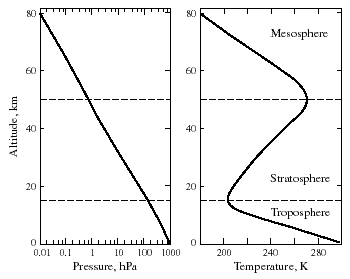
\includegraphics[scale=.85]{mecaflu/statiqueflu/polytrope.png}
    \vspace{-1.5em}
    \caption{Profils atmosphériques de pression et de température en fonction de l'altitude.}
\end{figure}
\end{itemize}
\end{exercise}